%!TEX root = ../thesis-main.tex

\chapter{Introduzione}\label{chap:introduction}
Il mondo del software ha scritto diverse decadi di storia. Sin dagli anni '50, quando i primi calcolatori programmabili hanno fatto il loro ingresso sul mercato, il software ha assunto un ruolo sempre più pervasivo nella vita quotidiana delle persone. Oltre ad essere parte integrante dei sistemi informativi delle aziende, lo possiamo trovare anche all'interno di automobili, elettrodomestici e tantissimi strumenti con la quale abbiamo a che fare nella nostra quotidianità. La crescente diffusione del software ha introdotto la necessità di progettare metodologie di sviluppo solide e versatili. Uno dei primi è il \textbf{modello a cascata} il quale struttura il processo di realizzazione del software in fasi sequenziali lineari. Il modello riprende la tipica organizzazione della produzione manifatturiera e fu progressivamente abbandonato con l'evolversi delle richieste del mercato. Successivamente prese piede il concetto di modelli iterativi come il \textbf{modello a spirale} in cui il processo di sviluppo è suddiviso in fasi multiple ripetute più volte (iterazioni). Gli ultimi decenni hanno dato vita a un nuovo modello, considerato lo standard dell'industria, la \textbf{metodologia agile}. Quest'ultima non rappresenta un unico modello, ma un insieme di modelli iterativi costruiti sulla base dei principi definiti all'interno del manifesto agile. Questi mettono in primo piano un ambiente autonomo e dinamico in cui sono fondamentali: cicli di sviluppo brevi, continui miglioramenti, la comunicazione col cliente e la consegna tempestiva di funzionalità. Il progetto esposto in questo documento introduce un evoluzione del concetto agile nato recentemente nel mondo dello sviluppo del software, conosciuto come ``DevOps".

\section{Contesto}
Con l'avvento di internet il concetto di software come un entità sviluppata e finita ha completamente cessato di esistere. Mediante la rete è diventato semplice ed efficiente distribuire un programma e fornire un ulteriore supporto attraverso aggiornamenti evolutivi e correttivi. Il fenomeno è cresciuto tanto da aver dato luce alla pratica del rilascio di applicazioni deliberatamente non complete, le quali attraverso il feedback degli utenti evolvono verso un prodotto finito. Il manifesto agile ha introdotto la cultura di emettere frequenti rilasci di nuove versioni del software, rendendo la distribuzione un punto cardine all'interno del ciclo di vita di esso. Dietro lo sviluppo rapido di nuove funzionalità è necessario il rilascio di queste altrettanto velocemente, la filosofia DevOps nasce per soddisfare questa esigenza.

\subsection{DevOps}
La metodologia DevOps (termine nato dalla contrazione di ``Development" ed ``Operations") si è formata intorno al 2008 con l'idea chiave di unire il team di sviluppo ed il team operativo (responsabile dell'infrastruttura del prodotto). Spesso accade all'interno di organizzazioni di grandi dimensioni che questi due componenti fondamentali siano separati, ossia il rilascio dell'applicazione avviene dopo che il processo di sviluppo è terminato, senza la possibilità tra i due di coordinarsi durante l'esecuzione. In sintesi, DevOps è molto più di una semplice pratica o metodologia; è una filosofia che promuove la collaborazione, l'automazione e il miglioramento continuo per garantire la distribuzione di software qualitativamente superiore.  
\begin{figure}[htb]
	\centering
	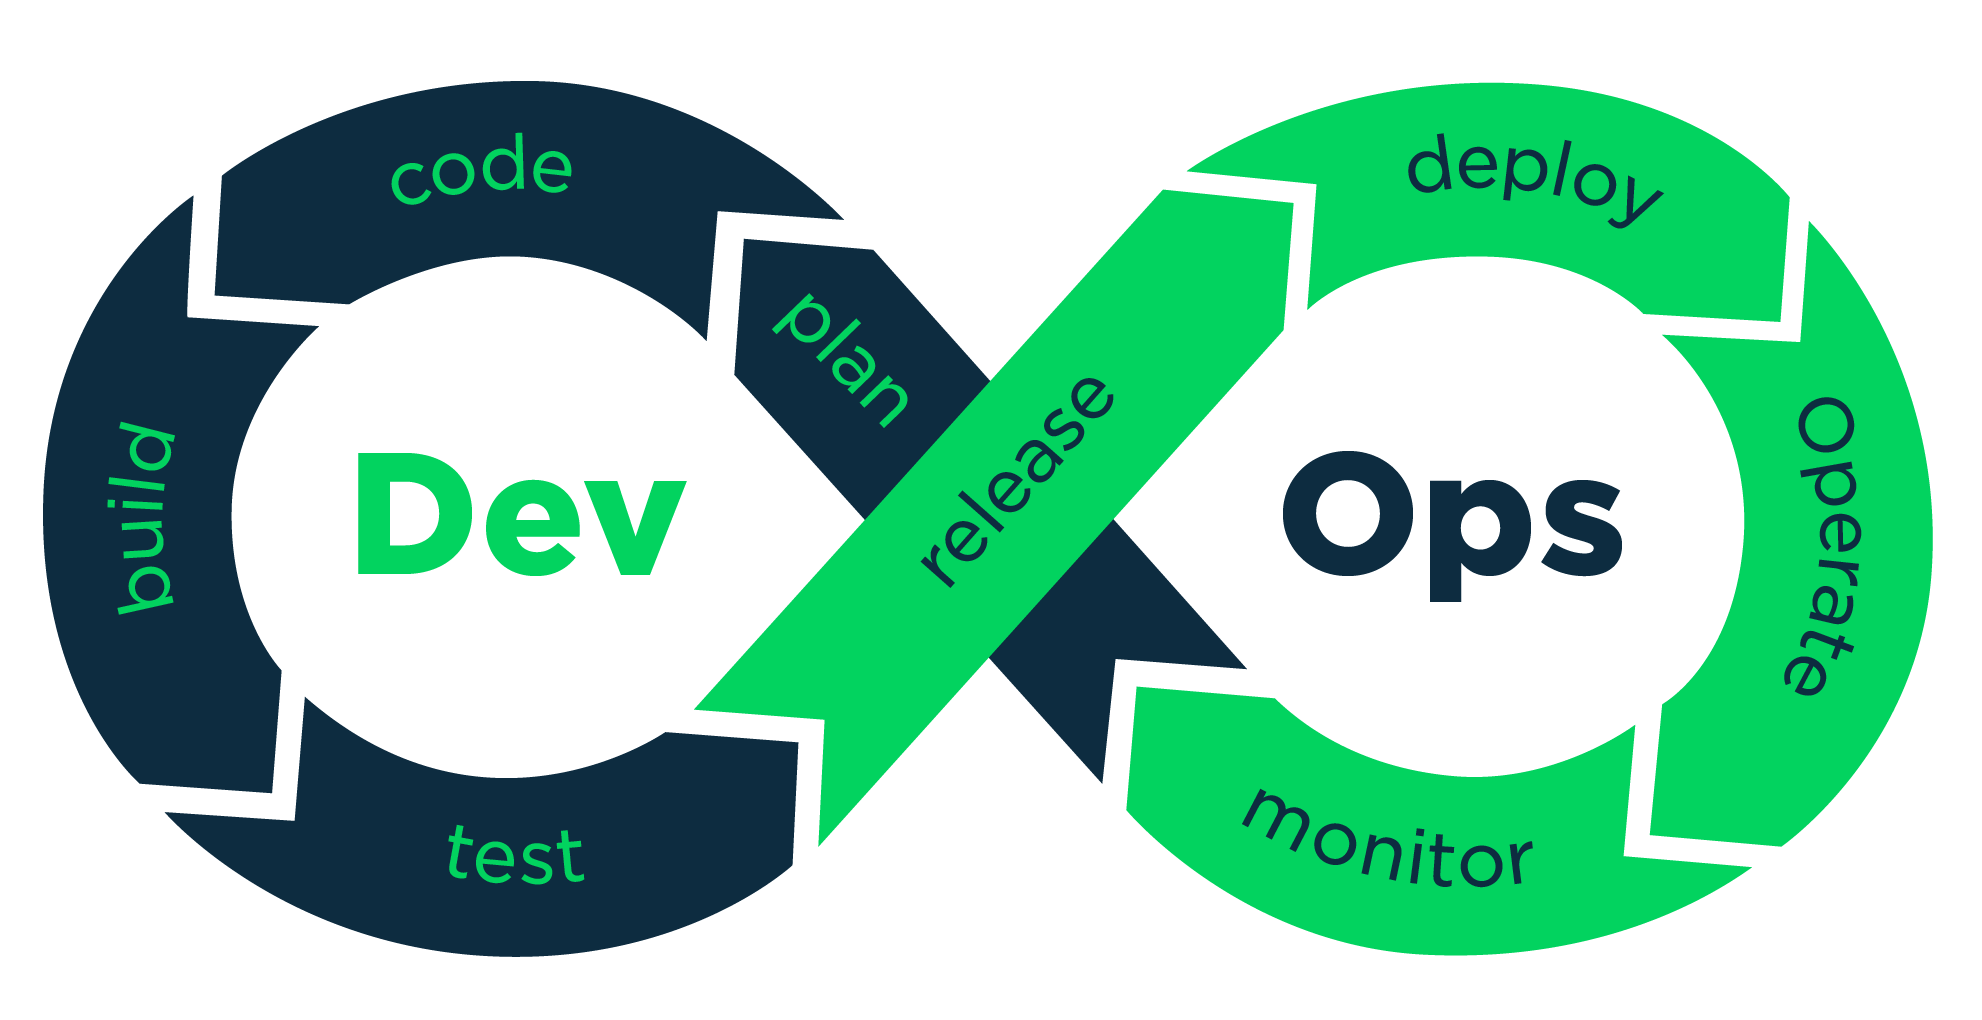
\includegraphics[width=.9\linewidth]{figures/devops-process.png}
	\caption{Le fasi della metodologia DevOps}
	\label{fig:devops-process}
	%https://italiancoders.it/introduzione-al-devops/
\end{figure}
Il modello illustrato nella figura \ref{fig:devops-process} suddivide un flusso in fasi distinte raggruppate per tipologia development oppure operations. È importante notare come la fine del flusso descritta dalla fase ``monitor" si collega nuovamente al ciclo successivo, ciò è dovuto al concetto di feedback continuo. Le metriche di prestazione e di utilizzo vengono monitorate costantemente per identificare i punti critici e migliorare le prestazioni del sistema in tempo reale. Questo ciclo di feedback consente alle organizzazioni di adattarsi rapidamente ai cambiamenti e di rispondere alle esigenze dei clienti in modo tempestivo.

Un altro concetto chiave è l'automazione. Automatizzare i processi ripetitivi riduce i potenziali errori e consente di monitorare in modo continuo il software. Questa caratteristica è ottenuta mediante lo sviluppo di pipeline di \ac{cicd}.

\paragraph{Continuous integration} La pratica della \textit{continuous integration} si concentra sull'integrazione automatica e continua delle modifiche al codice sorgente del progetto. Tipicamente, il processo si articola nei seguenti passaggi: (i) gli sviluppatori introducono nuovo codice nel progetto attraverso il software di \textit{version control}, (ii) un server acquisisce le modifiche, compila e testa l'intero progetto, (iii) una volta completato il processo, comunica agli sviluppatori l'esito delle operazioni. Questo approccio consente di individuare errori nel codice anticipatamente, garantendo stabilità e una maggiore qualità al software. Un aspetto fondamentale è la stesura dei test: un'eccessiva copertura può rallentare il processo di integrazione. È pertanto essenziale bilanciare la copertura dei test in base alle esigenze del progetto, tenendo presente che un aumento della copertura riduce il rischio di introdurre codice difettoso.

% Schema di una pipeline basilare

\paragraph{Continuous delivery} La distribuzione rappresenta l'insieme di operazioni finalizzate alla consegna del software agli utenti finali. Questo processo estende l'integrazione continua e si preoccupa di garantire la disponibilità costante di un artefatto di build pronto per il rilascio. L'effettivo rilascio di una nuova versione del software può avvenire in modo automatico oppure manualmente da parte dello sviluppatore; in merito non esistono regole stringenti, ogni progetto presenta esigenze differenti. La filosofia DevOps fornisce solamente linee guida capaci di fornire gli strumenti per progettare un processo di integrazione e distribuzione continua adeguato.

\subsection{Build automation}


\subsection{Un software complesso: Alchemist}\label{sec:alchemist}
Alchemist\cite{Pianini_2013} è un framework di simulazione open-source sviluppato dall'Università di Bologna, progettato per modellare elementi di programmazione pervasiva. Per comprendere l'ambito del progetto è necessario introdurre il concetto di simulazione in ambito scientifico. Per simulazione si intende un modello della realtà, costruito secondo le regole di un analista, sviluppato per consentire la valutazione dello svolgersi di una serie di eventi in un ambiente definito. Lo svolgimento di una simulazione avviene all'interno di un arco di tempo discreto suddiviso in unità di tempo predefinite definite come \textit{step}. Alchemist, consente di creare, osservare ed analizzare simulazioni atte a modellare interazioni tra agenti autonomi in ambienti dinamici: ossia scenari di \textit{aggregate} e \textit{nature-inspired computing}. Una rappresentazione del meta-modello, ossia le entità e relazioni configurabili, è raffigurata nella \cref{fig:alchemist-metamodel}.

\begin{figure}[htb]
	\centering
	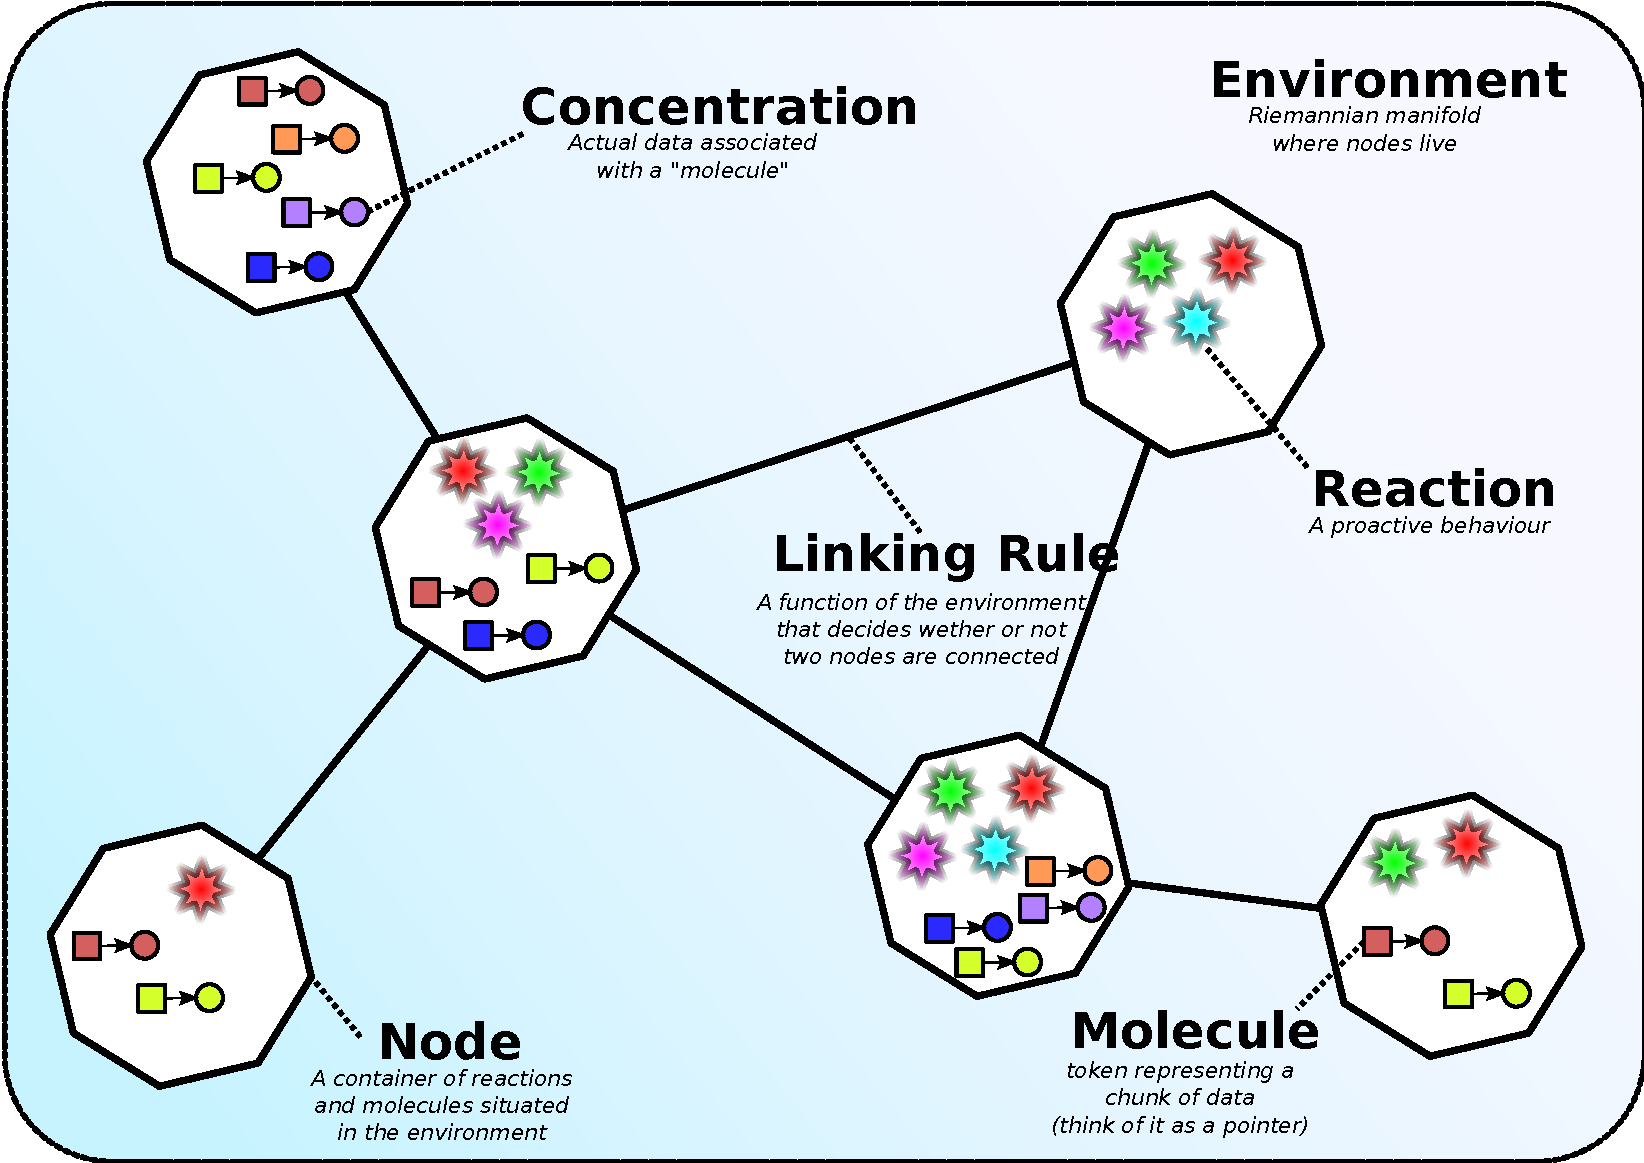
\includegraphics[width=.9\linewidth]{figures/alchemist-metamodel.pdf}
	\caption{Il meta-modello di Alchemist}
	\label{fig:alchemist-metamodel}
	%https://alchemistsimulator.github.io/explanation/metamodel/
\end{figure}

\paragraph{Architettura}
Il framework è realizzato mediante linguaggi \ac{jvm} (ossia eseguibili all'interno di macchine virtuali java), più precisamente Java e Kotlin, utilizzando una struttura modulare ed estendibile. L'intero motore di simulazione o le parti accessorie possono essere re-implementate senza modificare il modello ed allo stesso tempo il modello può essere esteso senza alterare il motore.

Il simulatore, come già citato, è un progetto open-source, ossia distribuito sotto termini di una licenza aperta. Questa permette a tutti di osservare il codice sorgente e di contribuire allo sviluppo del progetto, coordinato da un personale responsabile del suo avanzamento. La natura open-source del progetto apre le porte a modalità di sviluppo del codice differenti rispetto a team di dimensioni ridotte. In un progetto aperto i possibili sviluppatori che contribuiscono allo sviluppo sono potenzialmente infiniti, ragion per cui l'automazione è ancora più centrale e permette di tenere traccia della correttezza del codice fornito da utenti esterni. 


\subsection{Distribuzione del software}
% L'importanza del come si distribuisce il software
% Quanto capillarmente

\section{Obiettivi}
I punti discussi precedentemente hanno evidenziato l'importanza che l'automazione ricopre all'interno dello sviluppo del software. La tecniche descritte dalla filosofia DevOps eliminano l'intervento umano garantendo un maggior controllo sulla qualità del prodotto rilasciato. 

